\documentclass[german,aspectratio=169]{beamer}
\usetheme{Boadilla}

\definecolor{HSMblue}{rgb}{0.098,0.403,0.721} % HS Mainz (primary)
\usecolortheme[named=HSMblue]{structure}

% Frame title bit to the right
\makeatletter
\setbeamertemplate{frametitle}{%
	\ifbeamercolorempty[bg]{frametitle}{}{\nointerlineskip}%
	\@tempdima=\textwidth%
	\advance\@tempdima by\beamer@leftmargin%
	\advance\@tempdima by\beamer@rightmargin%
	\advance\@tempdima by-2.25cm% <- change value here
	\hfill%
	\begin{beamercolorbox}[sep=0.3cm,left,wd=\the\@tempdima]{frametitle}
		\usebeamerfont{frametitle}%
		\vbox{}\vskip-1ex%
		\if@tempswa\else\csname beamer@fteleft\endcsname\fi%
		\strut\insertframetitle\strut\par%
		{%
			\ifx\insertframesubtitle\@empty%
			\else%
			{\usebeamerfont{framesubtitle}\usebeamercolor[fg]{framesubtitle}\strut\insertframesubtitle\strut\par}%
			\fi
		}%
		\vskip-1ex%
		\if@tempswa\else\vskip-.3cm\fi% set inside beamercolorbox... evil here...
	\end{beamercolorbox}%
}
\makeatother

\setbeamersize{text margin left=1.5cm,text margin right=1.5cm}

% Input encoding
\usepackage[utf8]{inputenc} 

% Plots & Graphs
\usepackage{tikz}
\usetikzlibrary{shapes,arrows,snakes,decorations}
\usetikzlibrary{positioning,calc,fit}
\usetikzlibrary{backgrounds}
\usetikzlibrary{arrows.meta}
\usepackage{verbatim}


% Bibliography
\usepackage[backend=biber,style=numeric-comp,sorting=none]{biblatex}
\addbibresource{literature.bib}

\usepackage{caption}
\usepackage{subcaption}

\title[Realisierung einer CI/CD-Pipeline]{Realisierung einer CI/CD-Pipeline\\ für container-basierte verteilte Anwendungen}
\subtitle{Status Quo, Herausforderungen, Realisierung am konkreten Beispiel}
\author{Dr.-Ing. Stephan Schneider}

%\date{\today}
\date{Dezember 18, 2024}

\begin{document}
	\begin{frame}
\maketitle
\end{frame}
	
\begin{frame}
	\frametitle{Agenda}
	\tableofcontents
\end{frame}



	\begin{frame}
	\frametitle{Beispiel}
	\begin{center}
	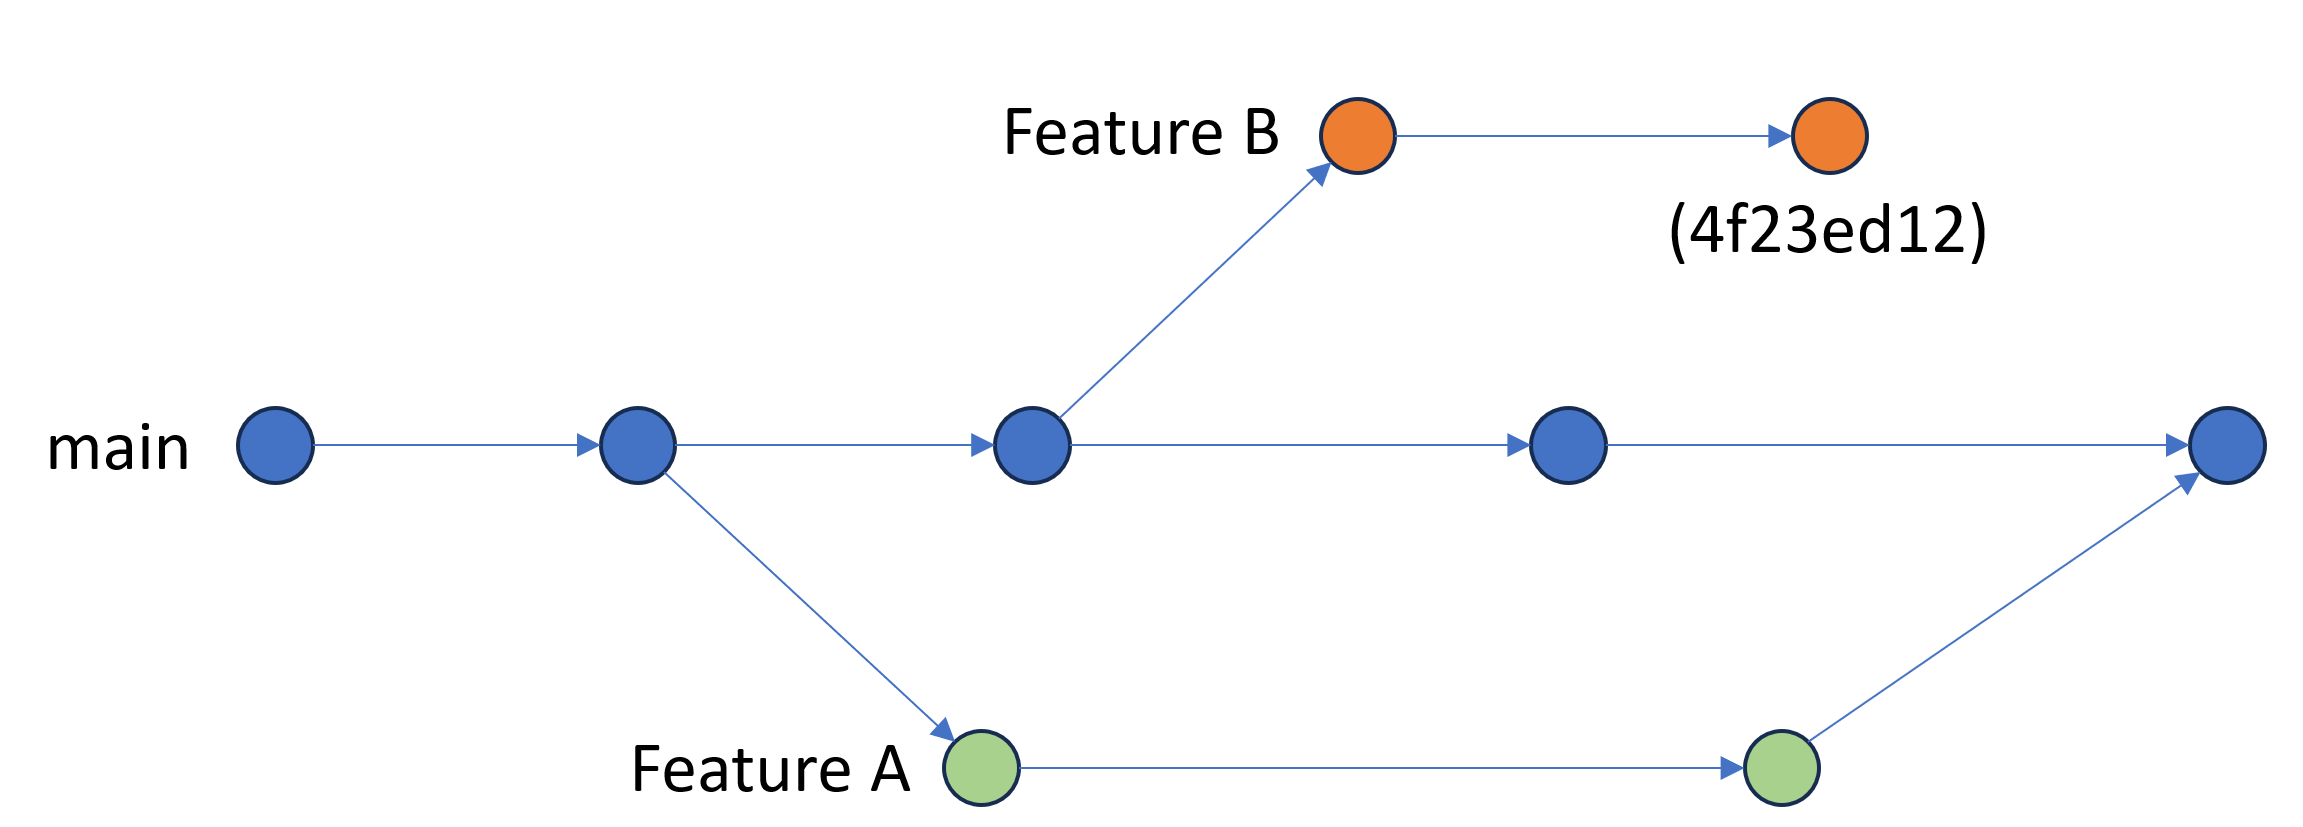
\includegraphics[width=0.95\textwidth]{img/git_history_01.png}
	\end{center}
\end{frame}

\begin{frame}
	\frametitle{Beispiel}
	\begin{center}
		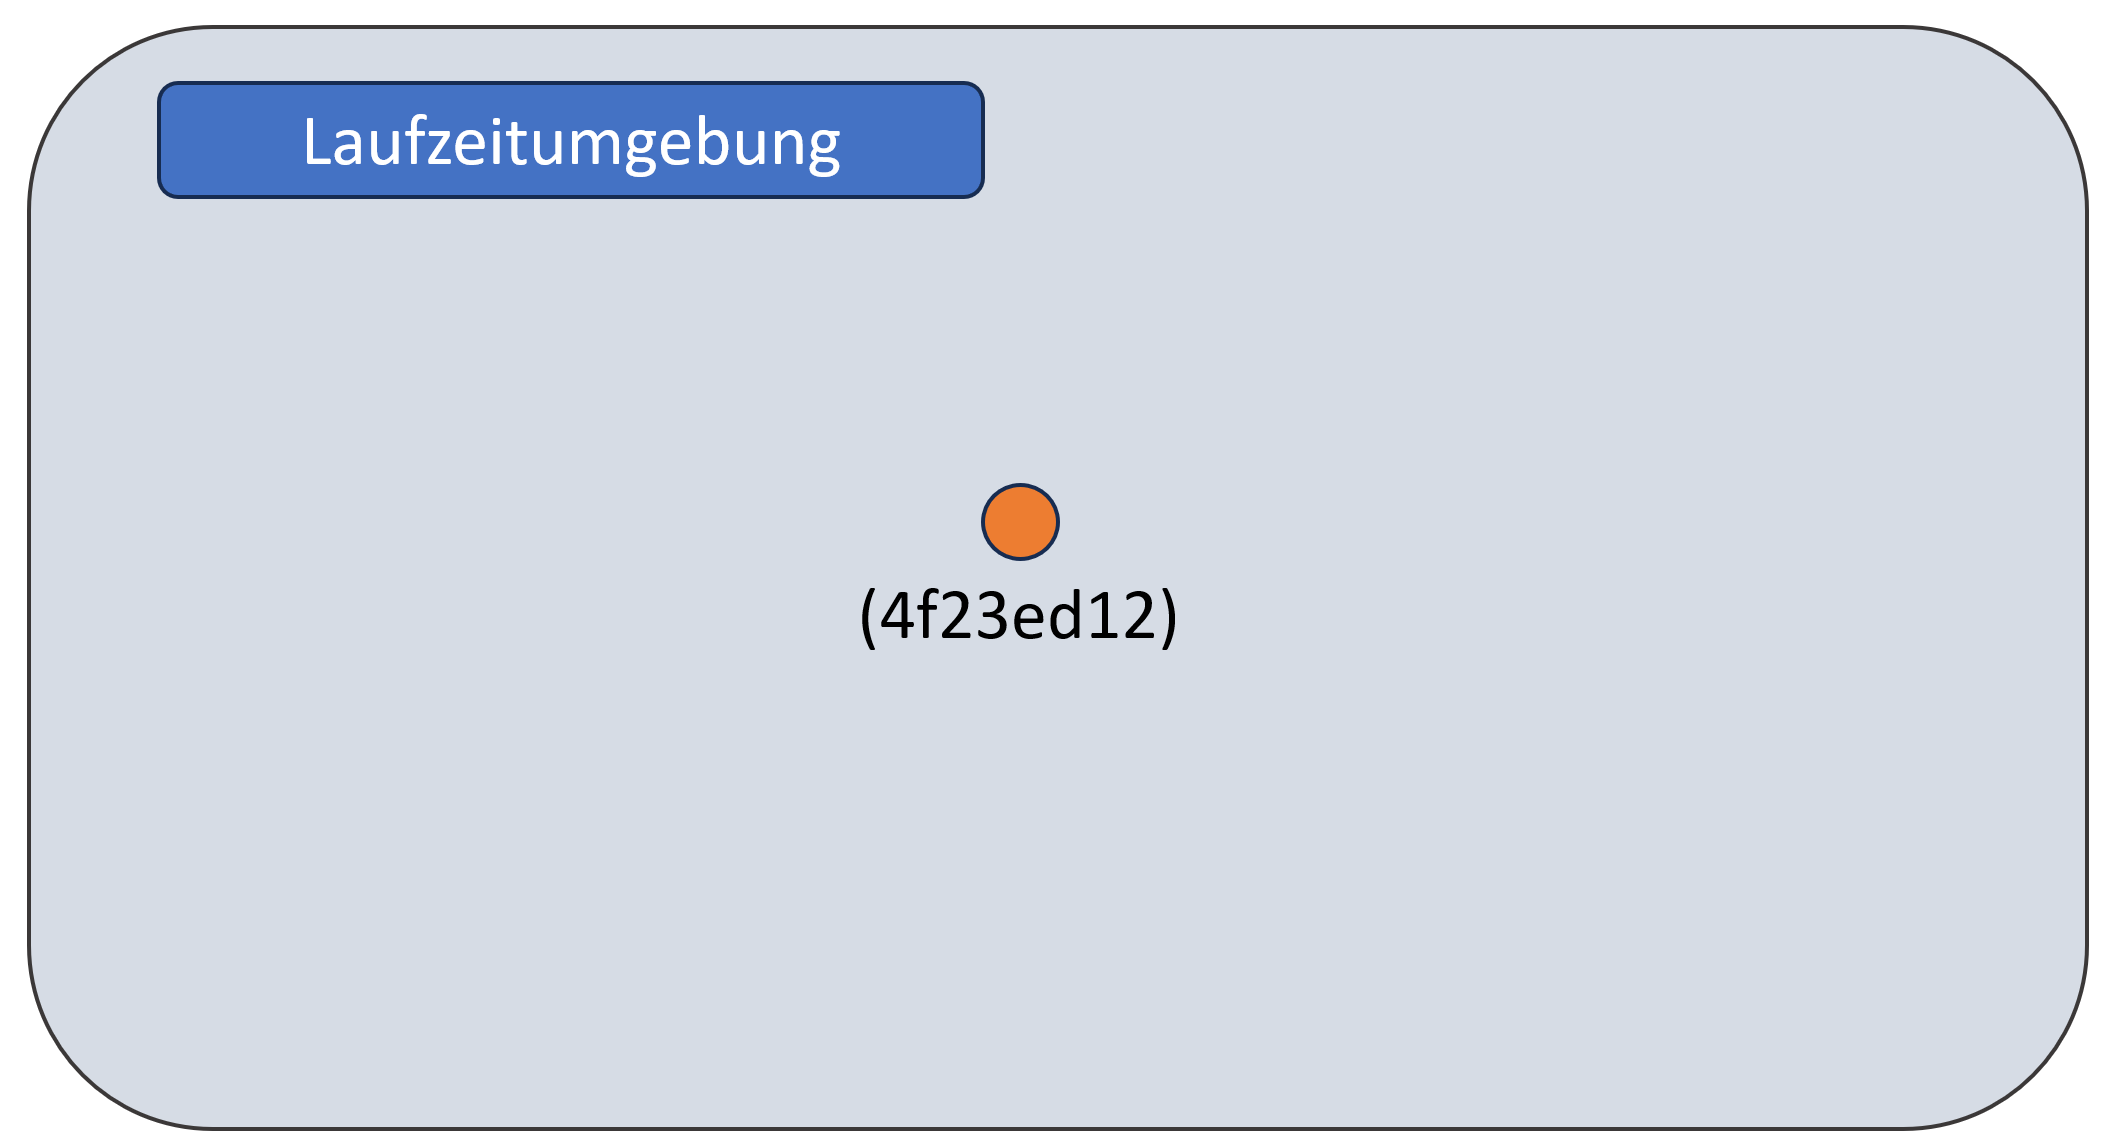
\includegraphics[width=0.95\textwidth]{img/environment_1.png}
	\end{center}	
	
\end{frame}

\begin{frame}
	\frametitle{Beispiel}	
	\begin{center}
		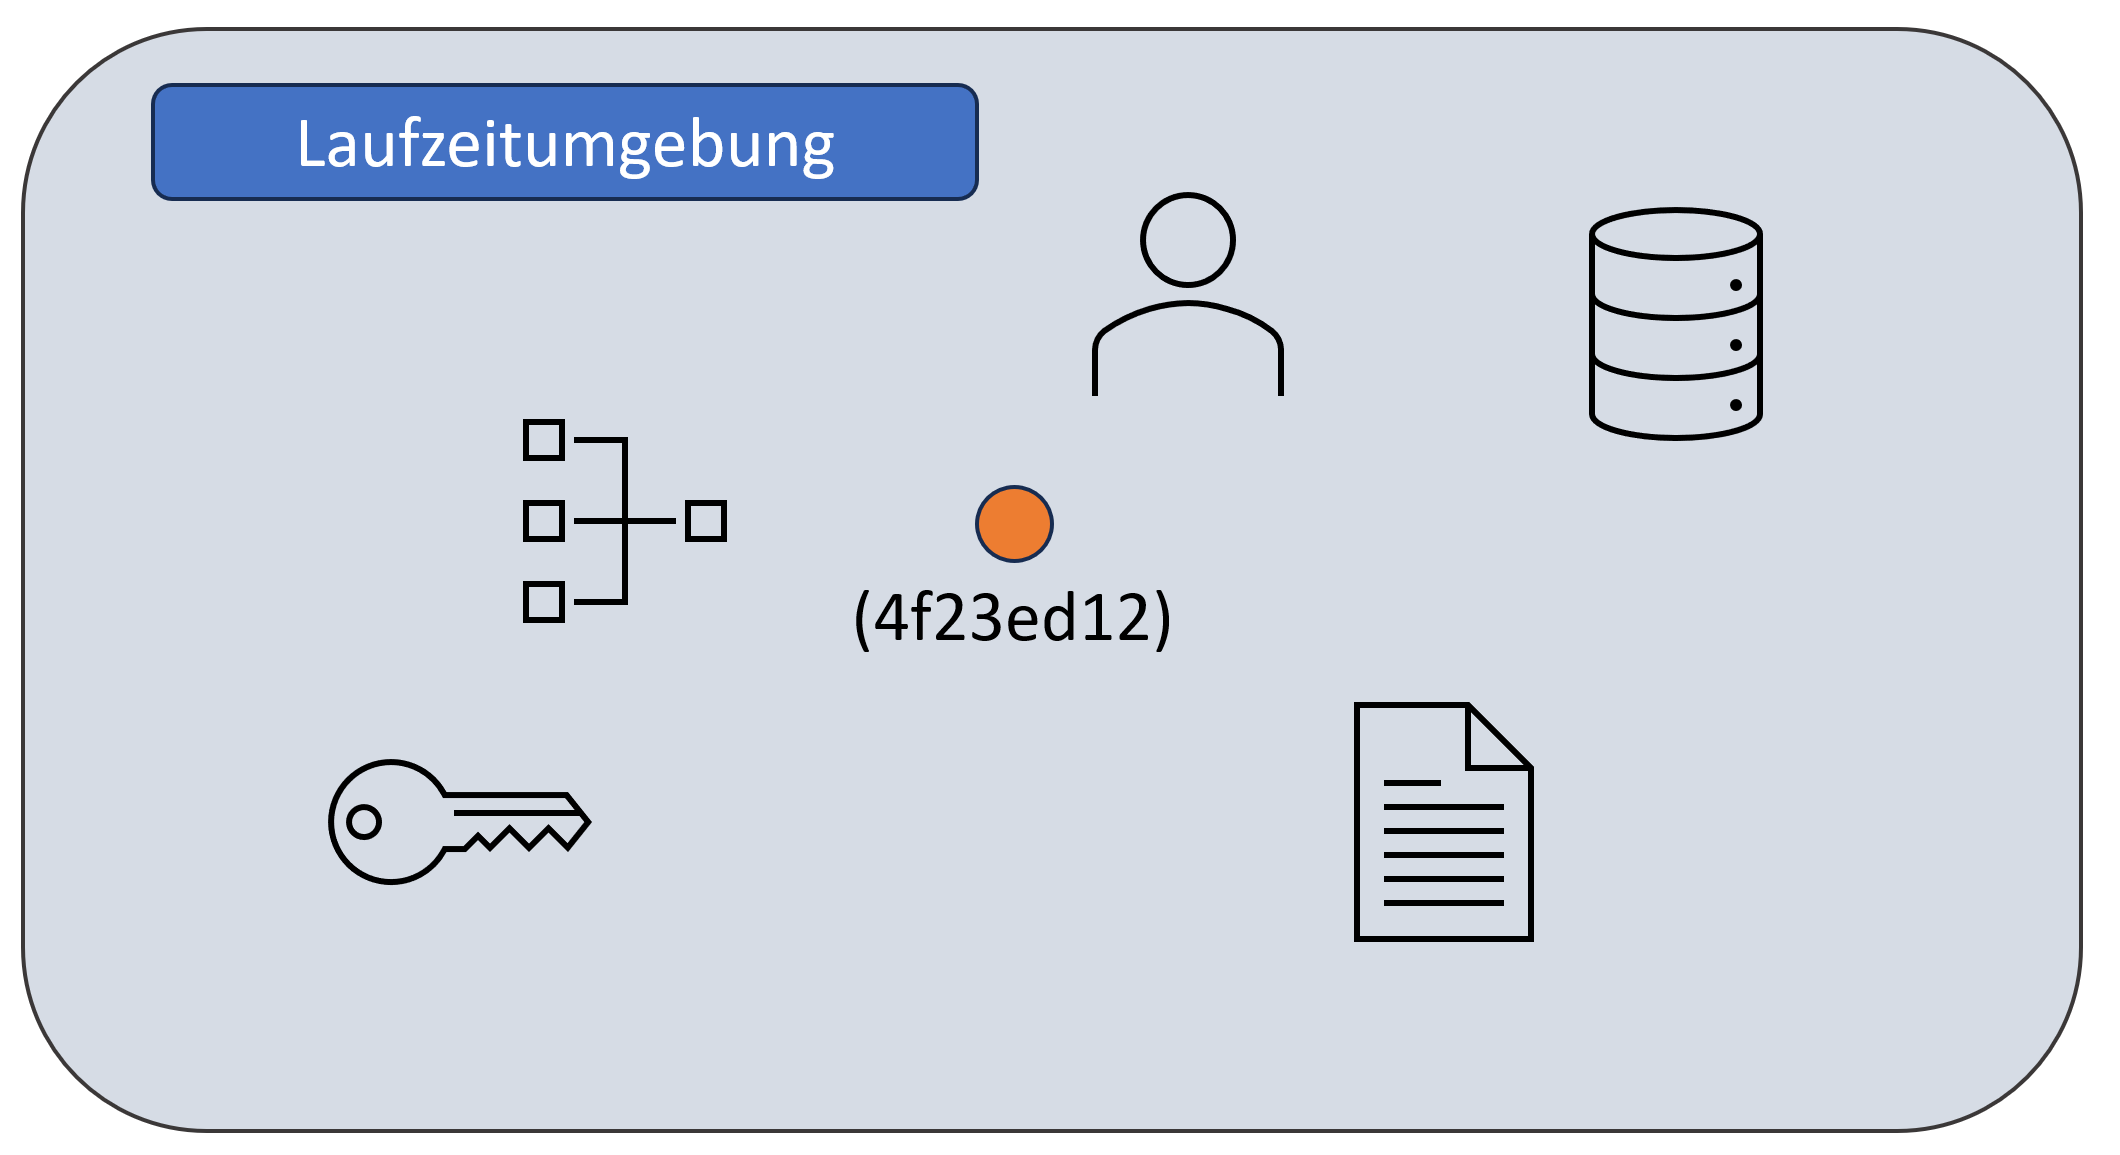
\includegraphics[width=0.95\textwidth]{img/environment_2.png}
	\end{center}
	
\end{frame}



	\section{Container-basierte Anwendungen}
	\begin{frame}
	\frametitle{Was sind Container?}
	\begin{definition}[Container]
		Eine Laufzeitumgebung einer Anwendung, mit allen notwendigen Abhängigkeiten.\\ 
	\end{definition}
	
	\begin{definition}[Image]
		Ein Image stellt die statische Abbildung des Dateisystems dar.
	\end{definition}
\end{frame}
	\begin{frame}
\frametitle{Container-basierte Anwendungen}

Was sind Container?
\begin{itemize}
	\item Leichtgewichtige Methoden zur Isolation von Dateisystemen, CPU- und Speicherressourcen, System- und Netzwerregeln
	\item Bieten jedoch eine geringere Isolation als virtuelle Systeme
\end{itemize}

\begin{columns}[T]
	\column{.5\textwidth}
	Vorteile:
	\begin{center}
		\begin{itemize}
			\item Geringer Overhead im Vergleich zu VMs
			\item Keine Hardware-Emulation
			\item Direkter Zugriff auf Ressourcen des Hostsystems (GPU, Netzwerk, Storage) 
		\end{itemize}
	\end{center}
	\column{.5\textwidth}
	Nachteile:
	\begin{center}
		\begin{itemize}
			\item Kein abweichendes OS möglich
			\item Keine Änderung der Kernelkonfiguration
			\item Schwache Isolation
		\end{itemize} 
	\end{center}
\end{columns}

\end{frame}




	\begin{frame}
	\frametitle{Container vs. Virtuelle Maschine}
	\begin{columns}
		\column{.5\textwidth}
		Container: \\
		\begin{center}
			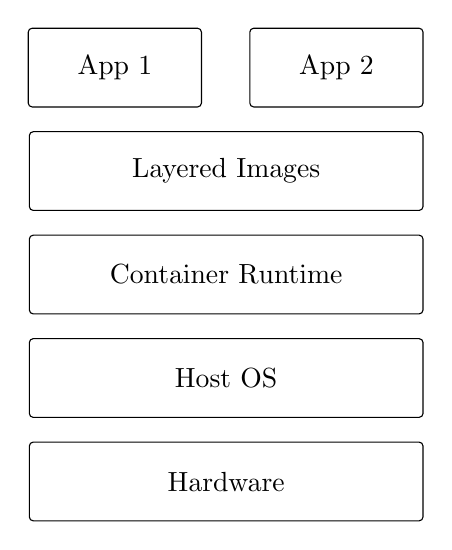
\begin{tikzpicture}
				\node[rectangle, draw, minimum width=5cm, minimum height=1cm,rounded corners=.05cm] (hardware) at (0,0) {Hardware};
				\node[rectangle, draw, minimum width=5cm, minimum height=1cm, above=0.3cm of hardware, rounded corners=.05cm] (os) {Host OS};
				\node[rectangle, draw, minimum width=5cm, minimum height=1cm, above=0.3cm of os, rounded corners=.05cm] (container) {Container Runtime};
				\node[rectangle, draw, minimum width=5cm, minimum height=1cm, above=0.3cm of container, rounded corners=.05cm] (image) {Layered Images};
				\node[rectangle, draw, minimum width=2.2cm, minimum height=1cm, above left=0.3cm and -2.2cm of image, rounded corners=.05cm] (apps1) {App 1};
				\node[rectangle, draw, minimum width=2.2cm, minimum height=1cm, right=0.6cm of apps1, rounded corners=.05cm] (apps2) {App 2};
			\end{tikzpicture}
		\end{center}
		\column{.5\textwidth}
		Virtuelle Maschine:\\
		\begin{center}
			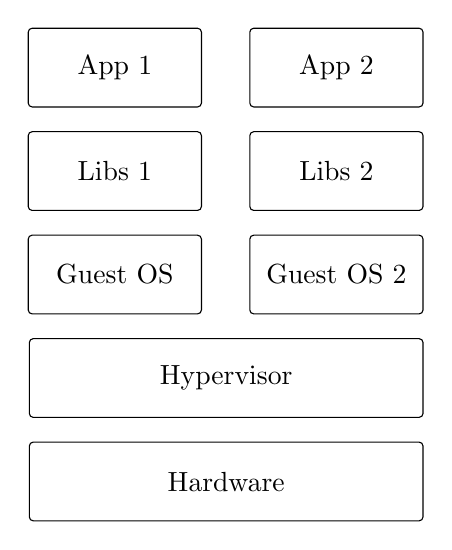
\begin{tikzpicture}
				\node[rectangle, draw, minimum width=5cm, minimum height=1cm,rounded corners=.05cm] (hardware) at (0,0) {Hardware};
				\node[rectangle, draw, minimum width=5cm, minimum height=1cm, above=0.3cm of hardware, rounded corners=.05cm] (hypervisor) {Hypervisor};
				\node[rectangle, draw, minimum width=2.2cm, minimum height=1cm, above left =0.3cm and -2.2cm of hypervisor, rounded corners=.05cm] (os1) {Guest OS};
				\node[rectangle, draw, minimum width=2.2cm, minimum height=1cm, right=0.6cm of os1, rounded corners=.05cm] (os2) {Guest OS 2};
				\node[rectangle, draw, minimum width=2.2cm, minimum height=1cm, above=0.3cm of os1, rounded corners=.05cm] (libs1) {Libs 1};
				\node[rectangle, draw, minimum width=2.2cm, minimum height=1cm, above=0.3cm of os2, rounded corners=.05cm] (libs2) {Libs 2};
				\node[rectangle, draw, minimum width=2.2cm, minimum height=1cm, above=0.3cm of libs1, rounded corners=.05cm] (apps1) {App 1};
				\node[rectangle, draw, minimum width=2.2cm, minimum height=1cm, above=0.3cm of libs2, rounded corners=.05cm] (apps2) {App 2};
			\end{tikzpicture}
		\end{center}
	\end{columns}
\end{frame}
	\begin{frame}
\frametitle{Layered Images}
\begin{columns}
	\column{.5\textwidth}
	\begin{center}	
	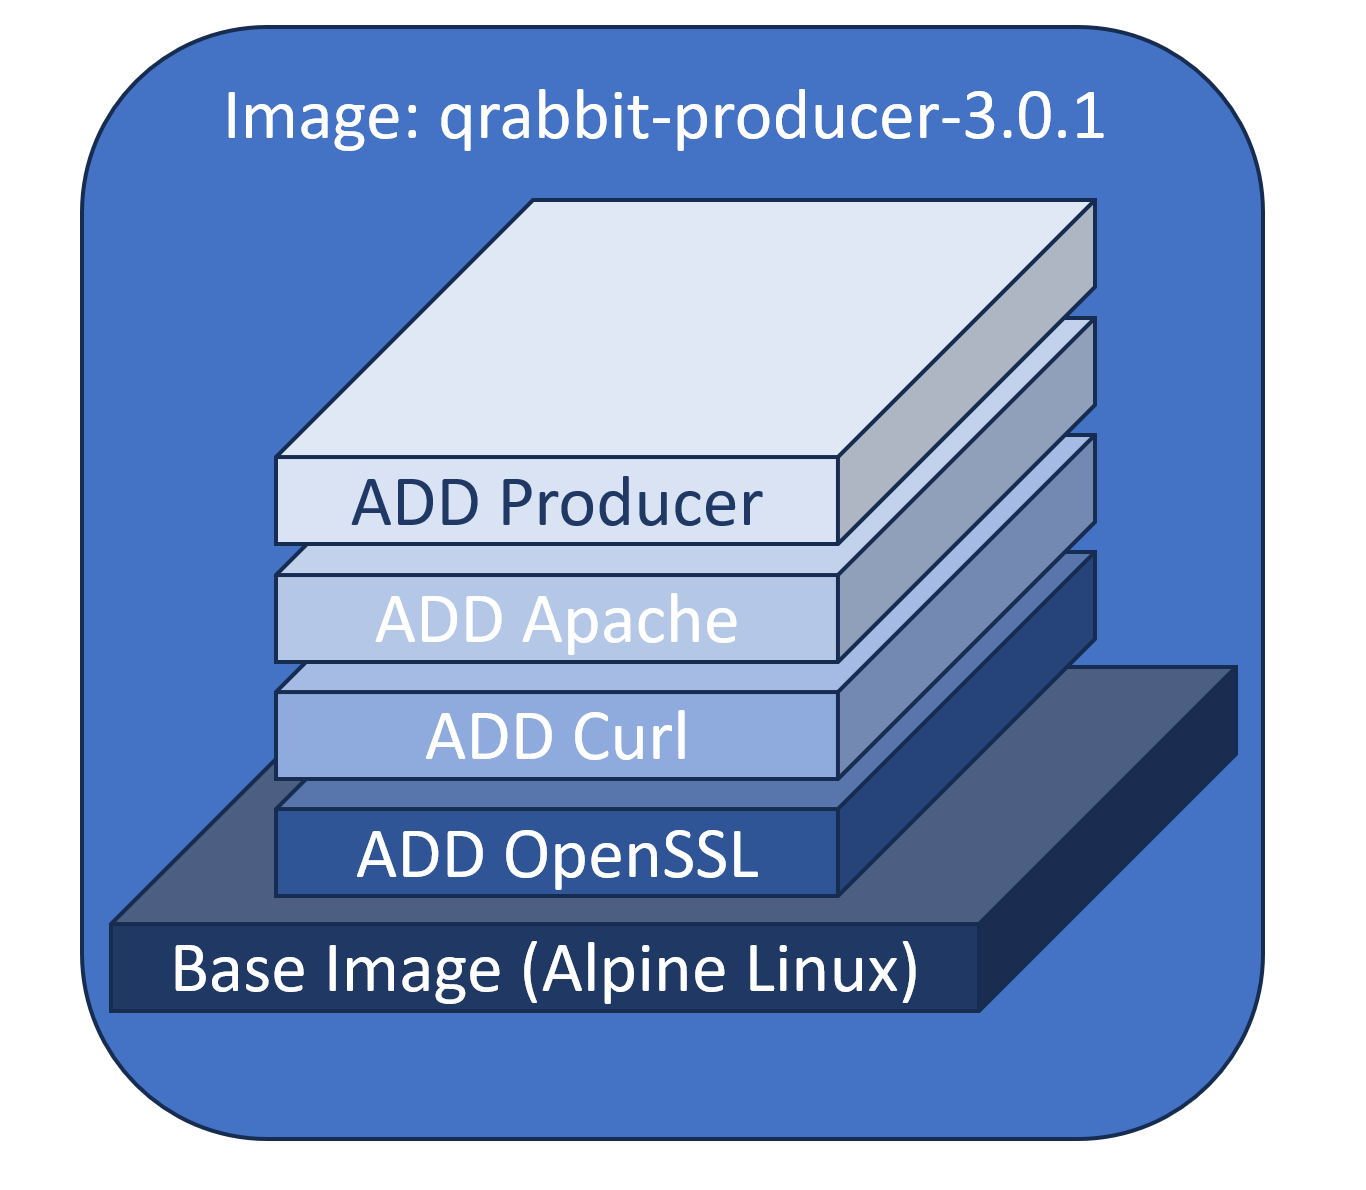
\includegraphics[width=0.98\textwidth]{img/image_01.png}
	\end{center}
	\column{0.5\textwidth}
	\begin{center}	
	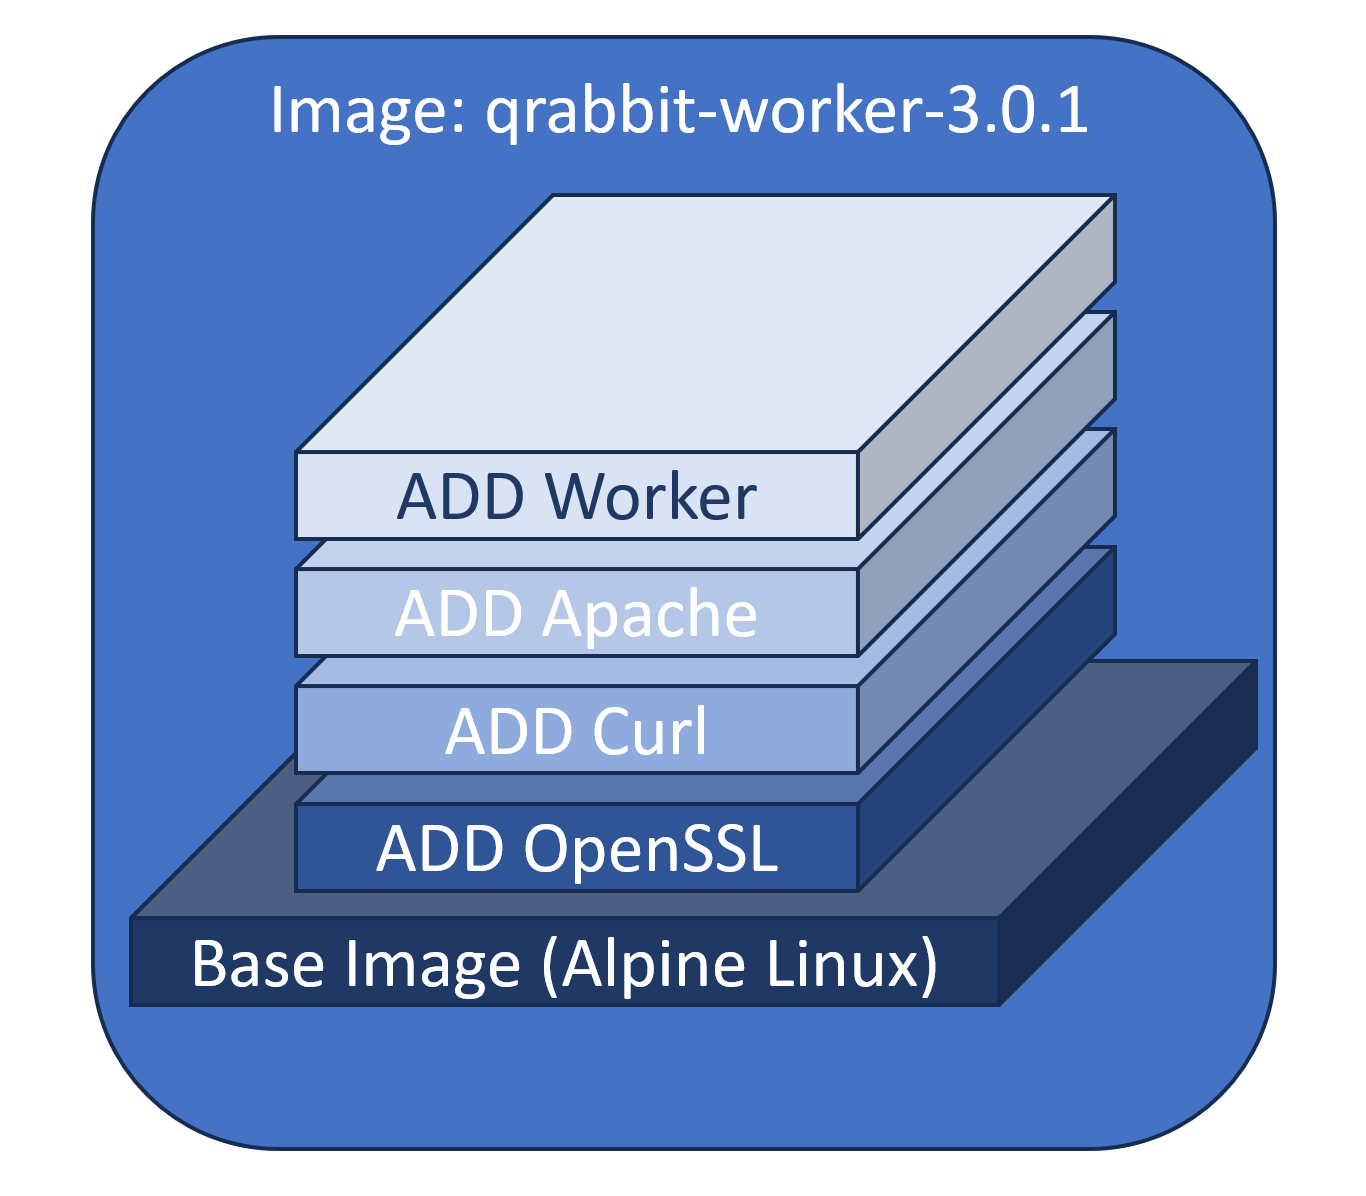
\includegraphics[width=0.98\textwidth]{img/image_02.png}
	\end{center}
\end{columns}
\end{frame}
	\begin{frame}
\frametitle{Docker}	
\begin{itemize}
	\item \textbf{1979} UNIX : \textit{chroot}
	\item \textbf{1999} BSD Jail
	\item \textbf{2000} Linux virtual environment
	\item \textbf{2004} Linux BSD Jail / Solaris Zones
	\item \textbf{2005} Linux OpenVZ
	\item \textbf{2008} Linux Containers (LXC)
	\item \textbf{2013} Docker (bis 2014 ein Wrapper für LXC)
\end{itemize}
\pause
Container sind keine neue Technologie und Docker ist nicht die einzige Container-Runtime. 
\end{frame}
	\begin{frame}
	\frametitle{Multilayer-Architektur}
	\begin{flushleft}
		
	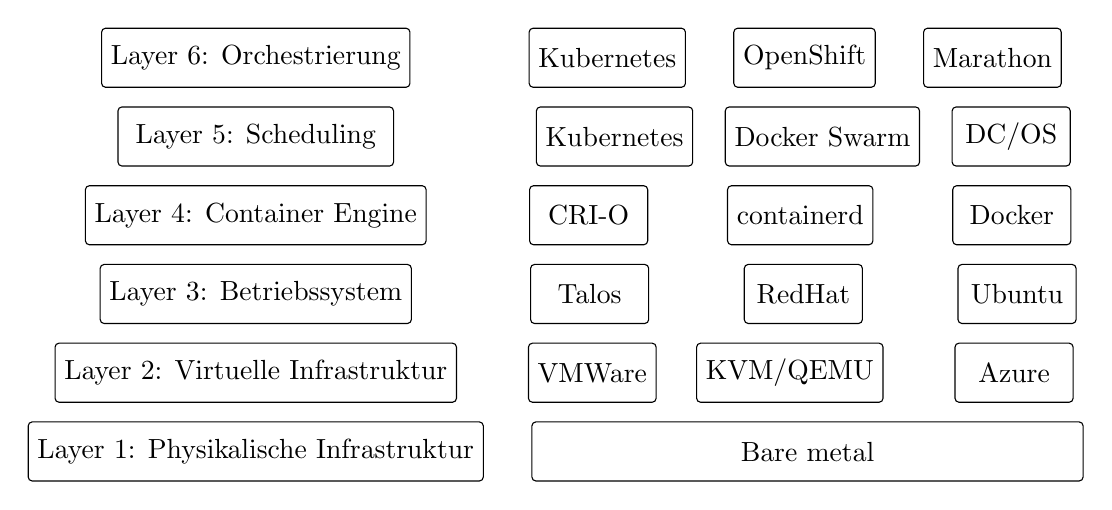
\begin{tikzpicture}
	
	\uncover<1->{
		\node[rectangle, draw, minimum width=3.5cm, minimum height=0.75cm,rounded corners=.05cm] (layer1) at (0, 0) {Layer 1: Physikalische Infrastruktur};
		\node[rectangle, draw, minimum width=7.0cm, minimum height=0.75cm,rounded corners=.05cm, right=3.5cm of layer1] (fe56) at (0, 0) {Bare metal};
	}
	\uncover<2->{
		\node[rectangle, draw, minimum width=3.5cm, minimum height=0.75cm,rounded corners=.05cm] (layer2) at (0, 1) {Layer 2: Virtuelle Infrastruktur};
		\node[rectangle, draw, minimum width=1.5cm, minimum height=0.75cm,rounded corners=.05cm, right=0.9cm of layer2] (vmware) {VMWare};
		\node[rectangle, draw, minimum width=1.5cm, minimum height=0.75cm,rounded corners=.05cm, right=0.5cm of vmware] (kvm) {KVM/QEMU};
		\node[rectangle, draw, minimum width=1.5cm, minimum height=0.75cm,rounded corners=.05cm, right=0.9cm of kvm] (azure) {Azure};
		
	}
	\uncover<3->{
		\node[rectangle, draw, minimum width=3.5cm, minimum height=0.75cm,rounded corners=.05cm] (layer3) at (0, 2) {Layer 3: Betriebssystem};
		\node[rectangle, draw, minimum width=1.5cm, minimum height=0.75cm,rounded corners=.05cm, right=1.5cm of layer3] (talos) {Talos};
		\node[rectangle, draw, minimum width=1.5cm, minimum height=0.75cm,rounded corners=.05cm, right=1.2cm of talos] (redhat) {RedHat};
		\node[rectangle, draw, minimum width=1.5cm, minimum height=0.75cm,rounded corners=.05cm, right=1.2cm of redhat] (ubuntu) {Ubuntu};
	}
	\uncover<4->{
		\node[rectangle, draw, minimum width=3.5cm, minimum height=0.75cm,rounded corners=.05cm] (layer4) at (0, 3) {Layer 4: Container Engine};
		\node[rectangle, draw, minimum width=1.5cm, minimum height=0.75cm,rounded corners=.05cm, right=1.3cm of layer4] (crio) {CRI-O};
		\node[rectangle, draw, minimum width=1.5cm, minimum height=0.75cm,rounded corners=.05cm, right=1.0cm of crio] (containerd) {containerd};
		\node[rectangle, draw, minimum width=1.5cm, minimum height=0.75cm,rounded corners=.05cm, right=1.0cm of containerd] (docker) {Docker};
	}
	\uncover<5->{
		\node[rectangle, draw, minimum width=3.5cm, minimum height=0.75cm,rounded corners=.05cm] (layer5) at (0, 4) {Layer 5: Scheduling};
		\node[rectangle, draw, minimum width=1.5cm, minimum height=0.75cm,rounded corners=.05cm, right=1.8cm of layer5] (k8s1) {Kubernetes};
		\node[rectangle, draw, minimum width=1.5cm, minimum height=0.75cm,rounded corners=.05cm, right=0.4cm of k8s1] (dockerswarm) {Docker Swarm};
		\node[rectangle, draw, minimum width=1.5cm, minimum height=0.75cm,rounded corners=.05cm, right=0.4cm of dockerswarm] (dcos) {DC/OS};
	}
	\uncover<6->{
		\node[rectangle, draw, minimum width=3.5cm, minimum height=0.75cm,rounded corners=.05cm] (layer6) at (0, 5) {Layer 6: Orchestrierung};
		\node[rectangle, draw, minimum width=1.5cm, minimum height=0.75cm,rounded corners=.05cm, right=1.5cm of layer6] (k8s2) {Kubernetes};
		\node[rectangle, draw, minimum width=1.5cm, minimum height=0.75cm,rounded corners=.05cm, right=0.6cm of k8s2] (openshift) {OpenShift};
		\node[rectangle, draw, minimum width=1.5cm, minimum height=0.75cm,rounded corners=.05cm, right=0.6cm of openshift] (marathon) {Marathon};
	}
			
	\end{tikzpicture}
	\end{flushleft}
	
\end{frame}
	\section{CI/CD Pipeline}
	\begin{frame}
\frametitle{CI/CD}

\begin{definition}
	\textbf{CI} : engl. \textit{Continious Integration}\\
	\textbf{CD} : engl. \textit{Continious Delivery} oder \textit{Continious Deploy} 
\end{definition}

\pause
Was soll kontinuierlich integriert werden?
\pause
\textbf{Softwareanpassungen!}\\
\pause 
Wo liegt der Unterschied zwischen \textit{Delivery} und \textit{Deploy}?\\
\pause
Beim Continious Delivery findet die Aktivierung im Produktivsystem manuell statt. 

\end{frame}

\begin{frame}
	\frametitle{Verfügbare CI/CD-Lösungen}
	\begin{itemize}
		\item Jenkins
		\item Gitlab 
		\item Travis-CI
		\item TeamCity
		\item CircleCI
		\item (uvm.)
	\end{itemize}
	Jede dieser Anwendungen besitze Stärken und Schwächen die im jeweiligen Projektkontext bewertet werden müssen. \\
	
	Die nachfolgenden Beispiele wurden mit GitLab und dessen CI/CD-Möglichkeiten erstellt.
\end{frame}

\begin{frame}
	\frametitle{CI/CD-Pipeline}
	\begin{center}
		\includegraphics[width=1.0\textwidth]{img/CI_CD_Example.png}
	\end{center}
\end{frame}
	\section{Beispielanwendung}
	\begin{frame}
\frametitle{Beispielanwendung}
\begin{itemize}
	\item Die Beispielanwendung besteht aus drei Java-Microservices
	\pause
	\item \textbf{Producer} erstellt Arbeitsaufträge und sendet diese an eine asynchrone Warteschlange. 
	\begin{itemize}
		\item<.-> \textbf{WAIT}: Kommando bewirkt einen Wartezyklus von 5~Sekunden im Worker
		\item<.-> \textbf{NOOP}: Kommando bewirkt eine Ausführung eines Nullbefehls
		\item<.-> \textbf{FIBONACCI}: Kommando bewirkt die Bereichnung einer Fibonacci-Zahl im Worker
		\item<.-> \textbf{KILL}: Kommando bewirkt, dass der Worker beendet wird.  
	\end{itemize}
	\pause
	\item \textbf{Worker} nimmt die Kommandos aus der Warteschlange und bearbeitet diese
	\begin{itemize}
		\item Abgearbeitete Kommandos werden in die Warteschlage \textbf{results} eingestellt 
	\end{itemize}
	\item \textbf{Writer} Der Prozess nimmt die Ergebnisse aus der Warteschlange \textbf{results} und persistiert diese.
\end{itemize}
\end{frame}

	\begin{frame}
	\frametitle{Beispielanwendung}
	
		\begin{center}
		\begin{tikzpicture}
			
			\uncover<0->{
				\node[rectangle, draw, minimum width=1.5cm, minimum height=1cm,rounded
				corners=.05cm] (producer) at (-5, 0) {Producer};
				\node[inner sep=0pt] (producerico) at (-5.85,0.5)
				{
\includegraphics[width=.05\textwidth]{img/png/resources/unlabeled/svc-256.png}};
			}
			
			\uncover<1->{
				\node[rectangle, draw, minimum width=1.5cm, minimum height=1cm,rounded
				corners=.05cm] (qrabbit1) at (-2, 0) {RabbitMQ $/$cmd};
				\node[inner sep=0pt] (cmdico) at (-3.45,0.5)
				{
\includegraphics[width=.05\textwidth]{img/png/resources/unlabeled/svc-256.png}};
				\draw[->] (producer.east) -- (qrabbit1.west);
			}
			
			\uncover<2->{
				\node[rectangle, draw, minimum width=1.5cm, minimum height=1cm,rounded
				corners=.05cm] (worker) at (1, 0) {Worker};
				\node[inner sep=0pt] (workerico) at (0.25,0.5)
				{
\includegraphics[width=.05\textwidth]{img/png/resources/unlabeled/svc-256.png}};
				\draw[->] (qrabbit1.east) -- (worker.west);
			}
			
			\uncover<3->{
				\node[rectangle, draw, minimum width=1.5cm, minimum height=1cm,rounded
				corners=.05cm] (qrabbit2) at (4, 0) {RabbitMQ $/$result};
				\node[inner sep=0pt] (qrabbit2ico) at (2.5,0.5)
				{
\includegraphics[width=.05\textwidth]{img/png/resources/unlabeled/svc-256.png}};
				\draw[->] (worker.east) -- (qrabbit2.west);
			}
			
			\uncover<4->{
				\node[rectangle, draw, minimum width=1.5cm, minimum height=1cm,rounded
				corners=.05cm] (writer) at (7, 0) {Writer};
				\node[inner sep=0pt] (writerico) at (6.25,0.5)
				{
\includegraphics[width=.05\textwidth]{img/png/resources/unlabeled/svc-256.png}};
				\draw[->] (qrabbit2.east) -- (writer.west);
			}
				
		\end{tikzpicture}
	\end{center}
\end{frame}
	
\begin{frame}
	\frametitle{Kubernetes Deployment}
	
	\begin{center}
		\begin{tikzpicture}
			
			\uncover<0->{
				% APPLICATION DEPLOYMENT
				\node[rectangle, draw, minimum width=10cm, minimum height=6.5cm,rounded corners=.05cm] (root) at (-0.5,1.5) {};	
				\node[inner sep=0pt] (ico) at (-5.5,4.75)
				{
\includegraphics[width=.05\textwidth]{img/png/resources/unlabeled/deploy-256.png}};
			}
				
%				% GITLAB

%				{
\includegraphics[width=.05\textwidth]{img/png/resources/unlabeled/deploy-256.png}};
%			}
%			
%			
			\uncover<1->{
				\node[rectangle, draw, minimum width=1.5cm, minimum height=1cm,rounded
				corners=.05cm] (workersvc) at (-0.5, 3.5) {Worker Service};
				\node[inner sep=0pt] (svcico) at (-1.75,4)				
				{
\includegraphics[width=.05\textwidth]{img/png/resources/unlabeled/svc-256.png}};
			}
%			
			\uncover<2->{
				
				\node[rectangle, draw, minimum width=1.5cm, minimum height=1cm,rounded
				corners=.05cm] (workerp1) at (-3.5, 1) {Worker Pod 1};
				\node[inner sep=0pt] (workerp1ico) at (-4.75,1.5)				
				{
\includegraphics[width=.05\textwidth]{img/png/resources/unlabeled/pod-256.png}};
				
				
				\node[rectangle, draw, minimum width=1.5cm, minimum height=1cm,rounded
				corners=.05cm] (workerp2) at (-0.5, 1) {Worker Pod 2};
				\node[inner sep=0pt] (workerp2ico) at (-1.75,1.5)				
				{
\includegraphics[width=.05\textwidth]{img/png/resources/unlabeled/pod-256.png}};
				
				\node[rectangle, draw, minimum width=1.5cm, minimum height=1cm,rounded
				corners=.05cm] (workerp3) at (2.5, 1) {Worker Pod 3};
				\node[inner sep=0pt] (workerp3ico) at (1.25,1.5)				
				{
\includegraphics[width=.05\textwidth]{img/png/resources/unlabeled/pod-256.png}};
				
				\node[rectangle, draw, minimum width=1.5cm, minimum height=1cm,rounded
				corners=.05cm] (workersec) at (-0.5, -1) {Worker Secret};
				\node[inner sep=0pt] (workersec) at (-1.75,-0.5)				
				{
\includegraphics[width=.05\textwidth]{img/png/resources/unlabeled/secret-256.png}};
			}
			
			\uncover<4->{
				\draw[->] (workerp1.north) -- (workersvc.south);
				\draw[->] (workerp2.north) -- (workersvc.south);
				\draw[->] (workerp3.north) -- (workersvc.south);
			}
%			
%			\uncover<3->{
%				% RUNNER
%				\node[rectangle, draw, minimum width=1.5cm, minimum height=1cm,rounded
%				corners=.05cm] (runner) at (-3, 1) {Runner};
%				\node[inner sep=0pt] (runnerico) at (-3.75,1.5)
%				
%				\draw[->] (gitlab.north) -- (runner.south) node[midway,fill=white] {Job};
%				
%			}
%			
%			\uncover<4->{
%				% REGISTRY
%				\node[rectangle, draw, minimum width=1.5cm, minimum height=1cm,rounded
%				corners=.05cm] (registry) at (0, 1) {Registry};
%				\node[inner sep=0pt] (registryico) at (-0.75,1.5)
%				{
\includegraphics[width=.05\textwidth]{img/png/resources/unlabeled/svc-256.png}};
%				\draw[->] (runner.east) -- (registry.west) node[midway,fill=white] {Store};
%			}
%			
%			
%			\uncover<5->{
%				% INTEGRATION REPOSITORY
%				\node[rectangle, draw, minimum width=1.5cm, minimum height=1cm,rounded
%				corners=.05cm] (intrepo) at (-8, 3) {Integration Repo.};
%				\draw[->] (runner.west) -- (intrepo.south east) node[midway,fill=white] {Trigger};		
%			}
%			
%			\uncover<6->{
%				% AGENT
%				\node[rectangle, draw, minimum width=1.5cm, minimum height=1cm,rounded corners=.05cm] (agent) at (0, 3) {Agent};
%				\node[inner sep=0pt] (agentico) at (-0.75,3.5)
%				{
\includegraphics[width=.05\textwidth]{img/png/resources/unlabeled/svc-256.png}};
%				\draw[->] (intrepo.east) -- (agent.west) node[midway,fill=white] {Trigger};
%			}			
%			
%			
%			\uncover<7->{
%				% APPLICATION
%				\node[rectangle, draw, minimum width=1.5cm, minimum height=1cm,rounded
%				corners=.05cm] (app) at (3, 1) {Application};
%				\node[inner sep=0pt] (appico) at (2,1.5)
%				{
\includegraphics[width=.05\textwidth]{img/png/resources/unlabeled/deploy-256.png}};
%				
%				\draw[->] (agent.east) -- (app.north) node[midway,fill=white] {Create};
%				\draw[->] (registry.east) -- (app.west) node[midway,fill=white] {Pull};			
%			}
%			
		\end{tikzpicture}
	\end{center}
\end{frame}


	\begin{frame}
	\frametitle{Übersicht Kubernetes}
	
	\begin{center}
		\begin{tikzpicture}

			\uncover<0->{
			% CLUSTER
			\node[rectangle, draw, minimum width=10cm, minimum height=6.5cm,rounded corners=.05cm] (root) at (-0.5,1.5) {};	
			\node[inner sep=0pt] (ico) at (-5.5,4.75)
			{
\includegraphics[width=.05\textwidth]{img/png/k8s.png}};
			
			
			% GITLAB
			\node[rectangle, draw, minimum width=1.5cm, minimum height=1cm,rounded
			corners=.05cm] (gitlab) at (-3, -1) {Gitlab};
			\node[inner sep=0pt] (gitlabico) at (-3.75,-0.5)
			{
\includegraphics[width=.05\textwidth]{img/png/resources/unlabeled/deploy-256.png}};
		}
			
			
			\uncover<1->{
				% DEVELOPER
				\node[rectangle, draw, minimum width=1.5cm, minimum height=1cm,rounded corners=.05cm] (dev) at (-8, 1) {Dev};	
			
				% GIT
				\node[rectangle, draw, minimum width=1.5cm, minimum height=1cm,rounded corners=.05cm] (git) at (-8, -1) {git};
				\draw[->] (dev.south) -- (git.north) node[midway,fill=white] {commit/push};					
				
			}
			
			\uncover<2->{
				\draw[->] (git.east) -- (gitlab.west) node[midway,fill=white] {push};
			}
			
			\uncover<3->{
				% RUNNER
				\node[rectangle, draw, minimum width=1.5cm, minimum height=1cm,rounded
				corners=.05cm] (runner) at (-3, 1) {Runner};
				\node[inner sep=0pt] (runnerico) at (-3.75,1.5)
				{
\includegraphics[width=.05\textwidth]{img/png/resources/unlabeled/svc-256.png}};
				\draw[->] (gitlab.north) -- (runner.south) node[midway,fill=white] {Job};
			
			}
			
			\uncover<4->{
			% REGISTRY
			\node[rectangle, draw, minimum width=1.5cm, minimum height=1cm,rounded
			corners=.05cm] (registry) at (0, 1) {Registry};
			\node[inner sep=0pt] (registryico) at (-0.75,1.5)
			{
\includegraphics[width=.05\textwidth]{img/png/resources/unlabeled/svc-256.png}};
			\draw[->] (runner.east) -- (registry.west) node[midway,fill=white] {Store};
			}
			
			
			\uncover<5->{
			% INTEGRATION REPOSITORY
			\node[rectangle, draw, minimum width=1.5cm, minimum height=1cm,rounded
			corners=.05cm] (intrepo) at (-8, 3) {Integration Repo.};
			\draw[->] (runner.west) -- (intrepo.south east) node[midway,fill=white] {Trigger};		
			}
			
			\uncover<6->{
			% AGENT
			\node[rectangle, draw, minimum width=1.5cm, minimum height=1cm,rounded corners=.05cm] (agent) at (0, 3) {Agent};
			\node[inner sep=0pt] (agentico) at (-0.75,3.5)
			{
\includegraphics[width=.05\textwidth]{img/png/resources/unlabeled/svc-256.png}};
			\draw[->] (intrepo.east) -- (agent.west) node[midway,fill=white] {Trigger};
			}			

			
			\uncover<7->{
			% APPLICATION
			\node[rectangle, draw, minimum width=1.5cm, minimum height=1cm,rounded
			corners=.05cm] (app) at (3, 1) {Application};
			\node[inner sep=0pt] (appico) at (2,1.5)
			{
\includegraphics[width=.05\textwidth]{img/png/resources/unlabeled/deploy-256.png}};
			
			\draw[->] (agent.east) -- (app.north) node[midway,fill=white] {Create};
			\draw[->] (registry.east) -- (app.west) node[midway,fill=white] {Pull};			
			}

		\end{tikzpicture}
	\end{center}
\end{frame}
	\section{Zusammenfassung}
	\begin{frame}
\frametitle{Summary}
\begin{itemize}
\item Using CI/CD-Pipelines is highly recommended to ensure nessecary software quality.
\pause
\item Modern container solutions provide
\begin{itemize}
	\pause
	\item Process isolation via kernel namespaces
	\pause
	\item Ressource constraints using kernel control groups
\end{itemize}
\pause
\item Implementing a reliable CI/CD operation many "moving" parts must align perfectly 
\pause
\end{itemize}
\end{frame}

\begin{frame}
	\begin{center}
		\begin{Huge}
			Thank you for your attention!
		\end{Huge}
		
		\vspace{1cm}
		
		GitHub: \url{https://github.com/p2k-ko/cicd_pipeline}\\
		
\includegraphics[width=0.35\textwidth]{img/github.png}
	\end{center}
\end{frame}
	\begin{frame}[allowframebreaks]
	\frametitle{References}
	\begin{itemize}
		\item K. Welter: \textit{Kubernetes}, 2024
		\item B. Öggl u. M. Kofler: \textit{Docker}, 2021
		\item O. Liebel: \textit{Skalierbare Container-Infrastrukturen, 4. Aufl.}, 2023
		\item A. Jones: \textit{Advanced GitLab CI/CD Pipelines}, 2024
		\item J. van Baarsen: \textit{Gitlab Cookbook}, 2014
		\item D. Dossot u. l. Johansson: \textit{RabbitMQ Essentials}, 2020
		\item M. Tefanko u. J. Martika: \textit{Quarkus in Action}, 2024
	\end{itemize}
	\nocite{*}
\end{frame}
\end{document}
